\documentclass[3p,times,twocolumn]{elsarticle}
\biboptions{numbers,sort&compress}
\usepackage[utf8]{inputenc}
\usepackage{doi}
%\setlength{\parskip}{0pt} % esp. entre parrafos
%\setlength{\parindent}{3pt} % esp. al inicio de un parrafo
\usepackage{amsmath} % mates
\usepackage{listings}
\usepackage[sort&compress,numbers]{natbib} % referencias
\usepackage{url} % que las URLs se vean lindos
\usepackage{hyperref} % ligas de URLs
\usepackage{graphicx} % poner figuras
\usepackage{subfigure}
\usepackage[spanish]{babel} % otros idiomas
\hypersetup{
    colorlinks=true,
    linkcolor=blue,
    filecolor=blue,      
    urlcolor=blue,
    citecolor=black,
}

\renewenvironment{abstract}{\global\setbox\absbox=\vbox\bgroup
  \hsize=\textwidth\def\baselinestretch{1}%
  \noindent\unskip\textbf{Resumen}  % <--- Edit as necessary
 \par\medskip\noindent\unskip\ignorespaces}
 {\egroup}

\def\keyword{%
  \def\sep{\unskip, }%
 \def\MSC{\@ifnextchar[{\@MSC}{\@MSC[2000]}}
  \def\@MSC[##1]{\par\leavevmode\hbox {\it ##1~MSC:\space}}%
  \def\PACS{\par\leavevmode\hbox {\it PACS:\space}}%
  \def\JEL{\par\leavevmode\hbox {\it JEL:\space}}%
  \global\setbox\keybox=\vbox\bgroup\hsize=\textwidth
  \normalsize\normalfont\def\baselinestretch{1}
  \parskip\z
  \noindent\textit{Palabras clave: }  % <--- Edit as necessary
  \raggedright                         % Keywords are not justified.
  \ignorespaces}
  
\title{Simulación del comportamiento de las nanopartículas ante concentraciones variables de solvente\tnoteref{t1}}
\tnotetext[t1]{Proyecto final de la materia Simulación Computacional de Nanomateriales}
\author[1]{Natalia Berenice Pérez López}
\ead{berenice_0112@hotmail.com}
\date{08 de diciembre de 2021}
\address[1]{Maestría en Ciencias de la Ingeniería con Orientación en Nanotecnología, \\ Facultad de Ingeniería Mecánica y Eléctrica, \\ Universidad Autónoma de Nuevo León}
\journal{Prof.\ Schaeffer for grading}

\begin{document}

\begin{abstract}
La nanotecnología actualmente está presente en más aspectos de la vida diaria de los que imaginamos, ésta ha sido clave en el desarrollo de nuevos materiales. Las nanopartículas tienen un diámetro inferior a cien nanómetros y debido a su tamaño tienen una relación entre área superficial y volumen muy elevada por lo que tienden a aglomerarse para reducir su energía superficial. Aplicar una agitación mecánica o utilizar como solvente etanol absoluto son algunas de las técnicas para evitar la aglomeración excesiva de las nanopartículas. En el presente trabajo se pretende simular el comportamiento de las nanopartículas al aplicar $5$\%, $25$\%, $50$\%, $75$\% y $98$\% de concentración del solvente, para así comparar y analizar la cantidad de nanopartículas iniciales y finales para cada concentración en un periodo de cien iteraciones.

\end{abstract}

\begin{keyword}
nanopartícula, aglomeración, solvente, simulación.
\end{keyword}

\maketitle

\section{Introducción}
Las aplicaciones potenciales de los nanomateriales incluyen su uso en
pigmentos para pinturas, catalizadores, productos farmacéuticos, baterías, celdas solares, dispositivos electrónicos y ópticos, memorias magnéticas de alta capacidad de almacenamiento, biomateriales, recubrimientos protectores, entre otros, de ahí su gran importancia de estudio y comprensión \cite{1}.
De manera general, los nanomateriales se pueden definir como materiales que poseen al menos una dimensión entre $1$ y $100$ nanómetros. Atendiendo a sus dimensiones podemos clasificar a los nanomateriales en cuatro categorías, considerando que un  nanomaterial $n$-dimensional es un material que tiene $n$ dimensiones mayores a $100$ nanómetros, tenemos los nanomateriales cero-dimensionales ($0$-D), monodimensionales ($1$-D), bidimensionales ($2$-D) y tridimensionales ($3$-D), estos últimos ya no serían propiamente nanomateriales, salvo que su estructura interna sea nanoestructurada \cite{2}.

Debido a su tamaño tan pequeño estos materiales pueden presentar distintas propiedades mecánicas, químicas, físicas, eléctricas, ópticas y catalíticas que el mismo material a una escala mayor. La adquisición de éstas propiedades únicas por parte de los nanomateriales es consecuencia del aumento significativo de la proporción del número de átomos que se encuentran en la superficie frente al número total de átomos en la partícula, lo cual también provoca que las partículas en la nanoescala sean más duras y reactivas que las mismas partículas a una escala mayor \cite{2}. Para obtener nanopartículas se tienen diferentes operaciones y procedimientos denominados métodos de síntesis, en los cuales se puede presentar un fenónemo muy común llamado aglomeración. En los procesos de síntesis de aerosoles las partículas se forman por nucleación y crecimiento, de manera que las nanopartículas en el rango de la nanoescala ($5$–$50$ nm) pueden formar conjuntos complejos químicamente unidos denominados agregados (rango de tamaño típico $200$–$300$ nm), los cuales a su vez, forman estructuras más grandes llamadas aglomerados que se mantienen unidos por fuerzas más débiles que surgen de la electrostática, Van der Waals, solvatación o efectos capilares. La aglomeración es un efecto no deseado que por lo general se busca evitar, para lograrlo es necesario estabilizar las nanopartículas individuales reduciendo su energía superficial libre. La presencia de agentes tensioactivos como ácidos y alcoholes, permiten estabilizar el crecimiento de las partículas y evitar la aglomeración.
 

\section{Antecedentes}\label{ant}

\subsection{Nanopartículas}
Las nanopartículas no necesariamente tienen que ser esferas perfectas, basta con cumplir con el requisito de tener sus tres dimensiones en la escala nanométrica para ser consideradas de ésta forma.

En los últimos años se han comercializado diferentes clases de nanopartículas, entre ellas las que se obtienen a partir del silicio, oro, dióxido de titanio, plata, óxido de zinc y de algunos otros materiales \cite{2}. A continuación se describen brevemente algunas de las aplicaciones de éstas nanopartículas:

\begin{enumerate}
    \item Nanopartículas de oro: Son ideales para absorber y dispersar la luz, también se utilizan para detectar tumores cancerígenos en el cuerpo de manera muy precisa.
    \item Nanopartículas de plata: Son utilizadas en aplicaciones sanitarias, al estar suspendidas en gel permiten tratar quemaduras y evitar infecciones.
    \item Nanopartículas de dióxido de titanio y óxido de zinc: Se utilizan en pastillas multivitamínicas, cremas solares, eliminación de bacterias en implantes ortopédicos, entre otras aplicaciones.
\end{enumerate}

Sin duda alguna hoy en día las nanopartículas representan un campo de estudio muy prometedor ya sea para encontrar nuevas aplicaciones o para mejorar sus aplicaciones actuales. 

\subsection{Fuerzas de Van der Waals}
Las fuerzas de Van der Waals son fuerzas intermoleculares de atracción o repulsión diferentes a las fuerzas de atracción electrostática y a las que generan los enlaces átomicos.

Como se mencionó anteriormente con la reducción del tamaño de las partículas a la escala nanométrica se incrementan las fuerzas de atracción de Van der Waals y las nanopartículas tienden a atraerse entre sí para aglomerarse y reducir su reactividad química. La energía de interacción total entre dos nanopartículas se puede calcular a partir de la contribución de las fuerzas de atracción y repulsión. Entre estas, se destaca la fuerza de atracción de Van der Waals, la cual es dependiente del radio de las partículas, la distancia de separación centro a centro, y la constante de Hamaker, representando éste último parámetro la atracción partícula-solvente-partícula \cite{3}.


\subsection{Métodos para evitar la aglomeración}
El grado de aglomeración de las nanopartículas se puede modificar o eliminar usando diferentes precursores, reactivos y solventes, o modificando los procesos de síntesis. Otro de los factores que afectan el grado de aglomeración de las nanopartículas es el tiempo que estas se hallan suspendidas en un solvente \cite{4}.

Las nanopartículas aglomeradas en un medio acuoso se pueden dispersar utilizando baños de ultrasonidos, sondas de ultrasonidos, agitadores magnéticos, molinos de bolas y homogeneizadores. La desaglomeración de las nanopartículas en líquidos dependerá del tiempo y de la intensidad de la energía utilizada para dispersar \cite{4}.

Es importante controlar la energía superficial de las nanopartículas ya que de lo contrario pueden seguir reaccionando y creciendo hasta formar aglomerados de tamaños lo suficientemente grandes para perder las propiedades únicas dependientes del tamaño nanométrico. 

\section{Trabajos relacionados}
Realizar un modelado de los procesos de aglomeración y agregación ímplica un reto muy desafiante cuando las partículas están en el rango de la nanoescala ($5$-$20$ nm), debido a que la física del sistema se encuentra entre la mecánica cuántica, la mecánica de partículas discretas y la mecánica continua.

Los modelos computacionales para simular el comportamiento dinámico de sistemas de partículas adhesivas se pueden clasificar en dos clases:
\begin{enumerate}
    \item Métodos basados en ecuaciones de equilibrio de población (PBE).
    \item Modelos de métodos de elementos discretos (DEM). 
\end{enumerate}
  
En general, el enfoque PBE es computacionalmente menos costoso, mientras que el enfoque DEM permite el uso de modelos más fundamentales. El método de elementos discretos fue desarrollado por Cundall y Strack en $1979$ para modelar sistemas granulares, posteriormente en el año de $1996$ Thornton, Yin y Adams utilizaron por primera vez un DEM para modelar partículas primarias que se agregan en un gran aglomerado \cite{5}.

En algunas simulaciones el elemento fundamental es una partícula primaria (PP), mientras que en otras aplicaciones se puede utilizar un agregado o incluso un aglomerado completo. Los modelos que consideran a las partículas primarias como elementos fundamentales se pueden utilizar para describir la formación de agregados, aglomerados y estructuras de películas delgadas \cite{5}.

\section{Modelo propuesto}\label{mod}
Para la simulación se propone un entorno bidimensional de dimensiones $10$ $\times$ $10$ en el cual se tienen $30$ nanopartículas, para fines prácticos los diámetros de cada nanopartícula se asignan al azar en un rango de $1$ a $5$ nanómetros y las posiciones $x$,$y$ así como su desplazamiento en dichos ejes también se eligen al azar para cada nanopartícula.

Para el movimiento de las nanopartículas dentro del cuadro delimitado se utiliza como base el movimiento del sistema multiagente revisado en clase durante la práctica \#6 \cite{6}. El tiempo del movimiento de las nanopartículas se mide en iteraciones, por lo cual para que se puedan apreciar las interacciones se estableció una simulación de $100$ iteraciones.

Se define un radio de acercamiento crítico, el cual indica la distancia máxima que puede haber entre dos nanopartículas, de tal manera que si una de ellas invade el radio crítico de otra nanopartícula ésta desaparece simulando la aglomeración entre ellas. 

Como se revisó en la sección \ref{ant} la aglomeración se puede evitar de distintas maneras, una de ellas es utilizando un solvente, por lo cual en la simulación se establecen cinco distintas concentraciones del solvente ($5\%$, $25\%$, $50\%$, $75\%$ y $98\%$). La concentración del solvente determina de manera probabilística si la nanopartícula que invadió el radio crítico de la otra nanopartícula se aglomerará con ella o no, por lo cual se espera que una mayor concentración de solvente evite mayormente la aglomeración al finalizar las iteraciones.

Para analizar estadísticamente el comportamiento de la simulación se realizan $10$ réplicas. Finalmente los resultados se analizan mediante gráficas de líneas y con un diagrama de violín combinado con caja-bigote. 

Las variables elegidas para la simulación del experimento se resumen en el cuadro \ref{Cuadro 1}.

\begin{table}[ht]
\centering
\begin{tabular}{ |p{4.2cm}||p{2.8cm}|}
 \hline
 \multicolumn{2}{|c|}{Datos del experimento} \\
 \hline
 Dimensión del cuadro & $10$ $\times$ $10$ \\
 \hline
 Nanopartículas    & $30$ \\
 \hline
 Réplicas    & $10$ \\
 \hline
 Iteraciones & $100$ \\
 \hline
  Radio crítico & 0.50 \\
 \hline
  Velocidad de desplazamiento& $1/10$ \\
 \hline
 Concentración del solvente & 0.05, 0.25, 0.50, 0.75, 0.98 \\
 \hline
\end{tabular}
\caption{Datos para la simulación.}
\label{Cuadro 1}
\end{table}


\section{Experimento}

\subsection{Código}
A continuación se muestra el fragmeto del código para definir los datos del experimento mostrados en el cuadro \ref{Cuadro 1}.

\definecolor{verde}{rgb}{0,0.56,0.22}
\definecolor{codegray}{rgb}{0.5,0.5,0.5}
\definecolor{codegreen}{rgb}{0,0.56,0.22}
\definecolor{backcolour}{rgb}{0.95,0.95,0.92}
\definecolor{azul}{rgb}{0,0,1}

\lstdefinestyle{mystyle}{
    backgroundcolor=\color{backcolour},   
    commentstyle=\color{verde},
    keywordstyle=\color{azul},
    numberstyle=\tiny\color{codegray},
    stringstyle=\color{codegreen},
    basicstyle=\ttfamily\footnotesize,
    breakatwhitespace=false,         
    breaklines=true,                 
    captionpos=b,                    
    keepspaces=true,                 
    numbers=left,                    
    numbersep=5pt,                  
    showspaces=false,                
    showstringspaces=false,
    showtabs=false,                  
    tabsize=2
}

\lstset{style=mystyle}
\begin{lstlisting}[language=R, caption= Fragmento del código para definir datos.]
l <- 10 #Dimension del cuadro bidimensional
n <- 30 #Cantidad de nanoparticulas
v <- 1 / 10 #Velocidad de desplazamiento
r <- 0.5 #Radio critico
concentracion = c(0.05, 0.25, 0.50, 0.75, 0.98) #Concentraciones del solvente
replicas = 10 #Cantidad de replicas
df = data.frame() 
\end{lstlisting}

Se agrega un ciclo \texttt{for} para variar las concentraciones del solvente, otro para hacer $10$ réplicas y uno más para crear las posiciones y diámetros de las $30$ nanopartículas. Además se agrega el código para crear un histograma de los tamaños de partícula y la gráfica del estado inicial del experimento.

\lstset{style=mystyle}
\begin{lstlisting}[language=R, caption= Fragmento del código para variar solvente y réplicas.]
for (solvente in concentracion){
  for (rep in 1:replicas){
    nanoparticulas <- data.frame(x = double(), y = double(),
                                 dx = double(), dy = double(), d = double())
    for (i in 1:n) {
      nanoparticulas <- rbind(nanoparticulas, data.frame(x = runif(1, 0, l),
                                                         y = runif(1, 0, l),
                                                         dx = runif(1, -v, v),
                                                         dy = runif(1, -v, v),
                                                         d = round(runif(1, 1, 5))))
    }
    
    tmax <- 100 #Cantidad de iteraciones
    digitos <- floor(log(tmax, 10)) + 1
    tl <- "0"
    while (nchar(tl) < digitos) {
      tl <- paste("0", tl, sep="")
    }
    png(paste("fig_00", tl, ".png", sep=""))
    plot(nanoparticulas$x, nanoparticulas$y, col=rainbow(20), pch=16, cex=nanoparticulas$d, xlim=c(-0.1, 10.1), ylim=c(-0.1, 10.1),
         main="Estado inicial", xlab="X", ylab="Y")
    graphics.off()
    
    png("Figura_1.png", width=15, height=15, units="cm", res=1200)
    ggplot(nanoparticulas, aes(x=d)) + geom_histogram(binwidth = 1, col='black', fill='blue')+
      labs(x = "Tamaño de particula (nm)", y = "Numero de particulas")+
      theme_bw()
    graphics.off() 
\end{lstlisting}

Enseguida se muestra el código para calcular la distancia entre dos nanopartículas, compararla con el radio crítico y decidir si se aglomeran o no tomando en cuenta la concentración del solvente. En el \texttt{data.frame} se almacena el número de réplica, el solvente y la cantidad de nanopartículas de cada iteración.

\begin{lstlisting}[language=R, caption= Fragmento del código para calcular distancia entre dos nanopartículas y decidir si se aglomeran.]
    for (tiempo in 1:tmax) {
      aglomeracion <- rep(FALSE, n)
      for (i in 1:n) { #Aglomeracion
        p1 <- nanoparticulas[i, ]
        for (j in 1:n) {
        if (!aglomeracion[j]) { #Aun se aglomera
            p2 <- nanoparticulas[j, ]
            dx <- p1$x - p2$x
            dy <- p1$y - p2$y
            dis <- sqrt(dx^2 + dy^2)
            if (dis < r) { #Radio critico
            aglomeracion[i] <- TRUE
            if (runif(1) > solvente){ #Solvente
                p1$d <- p1$d + p2$d
                p1 = p2
                nanoparticulas[i, ] <- p1 
              }
              nanoparticulas1 <- unique(nanoparticulas)
            }
          }
        }
      }
      parfinal = nrow(nanoparticulas1[nanoparticulas1$d,])
      result = c(solvente, rep, tiempo, parfinal)
      df = rbind(df, result)
\end{lstlisting}

El resto del código para el movimiento de las nanopartículas en el cuadro utilizando el método de \texttt{la dona} y el código para realizar las gráficas que se muestran en la sección \ref{res} se encuentran en \href{https://github.com/nataliaperez0/Simulation/tree/main/Proyectointegrador}{mi repositorio} en GitHub.

\subsection{Resultados}\label{res}

Primeramente podemos analizar el histograma del tamaño de partícula mostrado en la figura \ref{f1}. 

A continuación en la figura \ref{f2} se puede observar el comportamiento de las cinco curvas de acuerdo a la concentración del solvente, las cuales muestran la cantidad de nanopartículas en cada iteración. Para ésta gráfica solamente se realizó una réplica. 

Enseguida, en la figura \ref{f3} se puede observar una gráfica similar a la figura \ref{f2}, en ésta se muestra la cantidad de nanopartículas promedio de las $10$ réplicas en cada iteración. 

\begin{figure} [h!]% figura
    \centering
    \includegraphics[width=80mm]{Figura_1.png} % archivo
    \caption{Histograma del estado inicial del tamaño de nanopartícula.}
    \label{f1}
\end{figure} 

\begin{figure} [h!]% figura
    \centering
    \includegraphics[width=80mm]{Figura_22.png} % archivo
    \caption{Cantidad de nanopartículas en cada iteración para $1$ réplica.}
    \label{f2}
\end{figure} 

\newpage
\begin{figure} [h!]% figura
    \centering
    \includegraphics[width=80mm]{Figura_2.png} % archivo
    \caption{Cantidad promedio de nanopartículas en cada iteración para $10$ réplicas.}
    \label{f3}
\end{figure} 

Finalmente en la figura \ref{f4} se muestra un diagrama de violín combinado con caja-bigote para la cantidad de nanopartículas de acuerdo a la concentración del solvente. 

\begin{figure} [h!]% figura
    \centering
    \includegraphics[width=80mm]{Figura_3.png} % archivo
    \caption{Cantidad de nanopartículas para cada concentración del solvente.}
    \label{f4}
\end{figure} 

En la figura \ref{f5} se puede observar el estado inicial del cuadro bidimensional donde se encuentran las $30$ nanopartículas con diferentes tamaños, y en la figura \ref{f6} se muestra el mismo cuadro en la iteración número $100$.

\begin{figure} [h!]% figura
    \centering
    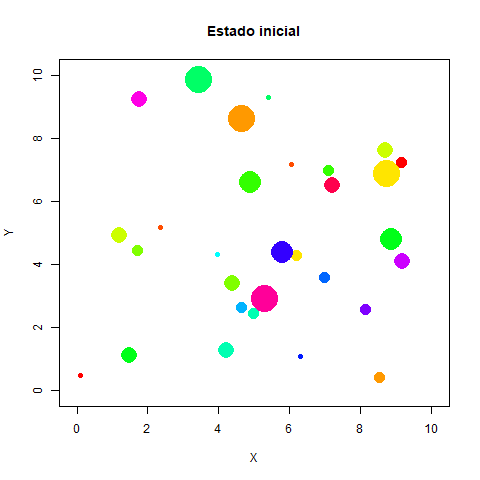
\includegraphics[width=80mm]{fig_00000.png} % archivo
    \caption{Estado inicial de las nanopartículas con un $5\%$ de concentración del solvente.}
    \label{f5}
\end{figure} 

\begin{figure} [h!]% figura
    \centering
    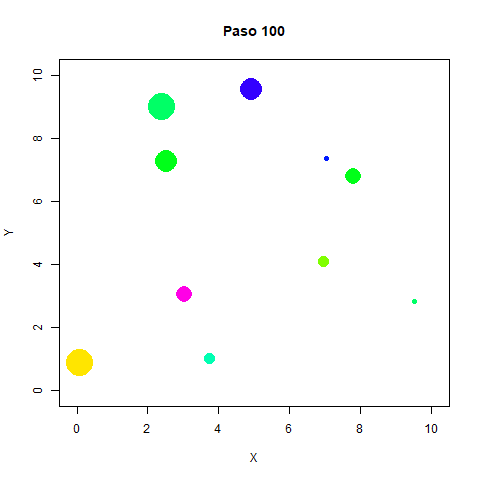
\includegraphics[width=80mm]{fig_100.png} % archivo
    \caption{Estado final o iteración número $100$ de las nanopartículas con un $5\%$ de concentración del solvente.}
    \label{f6}
\end{figure} 

En ésta última figura el tamaño de las nanopartículas debería ser mayor ya que se encuentran aglomeradas con las nanopartículas que ya no aparecen en la figura, sin embargo no se logró reflejar el tamaño para poder entender visualmente la aglomeración, solo se puede observar que hay una menor cantidad de nanpartículas que en el estado inicial.

En \href{https://github.com/nataliaperez0/Simulation/tree/main/Proyectointegrador/Gifs}{mi repositorio} se pueden encontrar los gifs con las $100$ iteraciones del experimento para cada concentración del solvente.

\subsection{Prueba estadística}
Para analizar si existe una relación entre la variación de la concentración del solvente y la cantidad final de nanopartículas se eligió realizar una prueba estadística.

En el cuadro \ref{Cuadro2} se  resumen los resultados de la revisión de los supuestos para poder aplicar la prueba estadística. El supuesto outliers se refiere a la cantidad de valores atípicos que existen en los grupos, la normalidad por grupos se obtuvo con la prueba de \texttt{Shapiro Wilk}, y la homogeneidad de varianza se obtuvo con la prueba de \texttt{Levene}.

\begin{table}[ht]
\centering
\caption{Resultados del los supuestos para aplicar la prueba estadística.}
\smallskip

\begin{tabular}{ |p{2.1cm}|p{3.5cm}|}
 \hline
 Outliers & $0$ \\
 \hline
 Normalidad por grupo & $0.05$: $p$ = $7.33\times 10^{-6}$ $0.25$: $p$ = $3.53\times 10^{-6}$ $0.50$: $p$ = $4.25\times 10^{-5}$ $0.75$: $p$ = $1.52\times 10^{-4}$ $0.98$: $p$ = $6.56\times 10^{-6}$ \\
 \hline
 Homogeneidad de varianza & $p$ = $8.69\times 10^{-16}$ \\
 \hline
\end{tabular}
\label{Cuadro2}
\end{table}

En los resultados se observa que ningún valor de $p$ es mayor a $0.05$, por lo tanto no tienen normalidad, cuando no se tiene normalidad en los grupos de datos la prueba estadística \texttt{Kruskal Wallis} es la adecuada. 

Al realizar la prueba \texttt{Kruskal Wallis} se obtienen los resultados mostrados en el cuadro \ref{Cuadro3}.

\begin{table}[ht]
\centering
\caption{Resultados al aplicar la prueba estadística \texttt{Kruskal Wallis}.}
\smallskip

\begin{tabular}{ |p{2.1cm}|p{2.1cm}|}
 \hline
 Chi cuadrada & Valor de $p$ \\
 \hline
 $219.57$ & $2.2\times 10^{-16}$ \\
 \hline
\end{tabular}
\label{Cuadro3}
\end{table}

Hipótesis nula : Las medias son iguales en todos los grupos.
\smallskip

Hipótesis alternativa: Debido a que $p < 0.05$ se rechaza la hipótesis nula, es decir que si existen diferencias significativas entre las medias de los grupos. 
\smallskip

Se entiende entonces que la variación de la concentración del solvente si tiene un efecto significativo en la cantidad final de nanopartículas. 

Aplicando la prueba de suma de rangos de \texttt{Wilcoxon} por pares, podemos observar los resultados de $p$ y determinar si existen diferencias al comparar entre ellas cada una de las muestras (Ver cuadro \ref{Cuadro4}).

\begin{table}[ht]
\centering
\caption{Resultados al aplicar la prueba \texttt{Wilcoxon}.}
\smallskip

\begin{tabular}{|p{1.5cm}|p{1.2cm}|p{1.2cm}|p{1.2cm}|p{1.2cm}|}
 \hline
Valor de $p$ & $0.05$ & $0.25$ & $0.50$ & $0.75$\\
 \hline
 $0.25$ & $1$ & - & - & - \\
 \hline
 $0.50$ & $1$ & $1$ & - & -\\
 \hline
  $0.75$ & $0.117$ & $0.007$ & $0.064$ & - \\
 \hline
  $0.98$ & $2\times 10^{-16}$ & $2\times 10^{-16}$ & $2\times 10^{-16}$ & $2\times 10^{-16}$ \\
 \hline
\end{tabular}
\label{Cuadro4}
\end{table}

En los resultados de la prueba podemos ver que las comparaciones de $0.05$ con $0.25$, $0.05$ con $0.50$ y $0.25$ con $0.50$ tienen una $p > 0.05$, por lo tanto se puede determinar que solamente en estas muestras no existen diferencias entre ellas. 

A continuación se muestra el código utilizado para realizar la prueba estadística \texttt{Kruskal Wallis}:

\lstset{style=mystyle}
\begin{lstlisting}[language=R, caption= Código para graficar y realizar la prueba estadística \texttt{Kruskal Wallis}.]
library(tidyverse)
library(ggpubr)
library(car)
library(rstatix)
library(rapportools)
library(readr)
library(gridExtra)

#PRUEBA ESTADISTICA...
#Estadisticas descriptivas
df2 %>%
  group_by(Sol) %>%
  get_summary_stats(NPs, type = "mean_sd")

#SUPUESTOS PARA ANOVA
#1:Outliers
df2 %>%
  group_by(Sol) %>%
  identify_outliers(NPs)

#2:Normalidad por Shapiro
tapply(df2$NPs, df2$Sol, shapiro.test)

#3:Homogeneidad de varianza con prueba Levene
df2 %>%
  levene_test(NPs~Sol)

#PRUEBA ESTADISTICA KRUSKAL WALLIS
kruskal.test(NPs ~ Sol, data = df2)

#PRUEBA WILCOXON
pairwise.wilcox.test(df2$NPs, df2$Sol)
\end{lstlisting}

\subsection{Discusión}
En la figura \ref{f1} podemos observar que el tamaño de las nanopartículas iniciales no presenta una distribución normal y este comportamiento es lógico porque al asignar los diámetros a cada nanopartícula se elegió una distribución uniforme y no normal. Tanto en la figura \ref{f2} como en la figura \ref{f3} se observa un comportamiento similar, solo que en la figura \ref{f2} el comportamiento se aprecía más marcado y no suavizado como en la figura \ref{f3} ya que ésta última utiliza el promedio de las $10$ réplicas. Los resultados observados son los esperados ya que cuando se tiene una mayor concentración del solvente es menos probable que las nanopartículas se aglomeren. En la figura \ref{f4} se visualiza de mejor manera las diferencias entre las cantidades de nanopartículas para cada concentración del solvente.

\section{Conclusiones}
Con base en las gráficas obtenidas y la prueba estadística aplicada es posible concluir que la variación de la concentración del solvente puede ayudar a evitar o controlar el crecimiento de las nanopartículas para así mantenerlas dentro de la escala nanométrica y no perder sus propiedades dependientes del tamaño. De está manera también se puede comprender la importancia de los métodos de síntesis para obtener nanopartículas estables para así poder controlar adecuadamente su tamaño.

\section{Trabajo futuro}
Dado que la nanotecnología tiene muchas aportaciones por hacer es importante enfrentar los retos que supone, como es el caso del control adecuado del tamaño o los efectos en la salud de los seres humanos. Considero que la simulación de estos fenómenos son de gran ayuda para comprender y proponer soluciones a éstos retos. En esta simulación no se logró representar visualmente el fenómeno de la aglomeración como tal, por lo que sigue representando trabajo futuro para lograrlo, además se tienen muchos otros parámetros que por cuestiones de simplicidad no se tomaron en cuenta como es el caso de la energía superficial presente en las nanopartículas, por lo que realizar una simulación más completa tomando en cuenta más parámetros reales también suponen trabajo futuro.

\newpage

\bibliographystyle{elsarticle-num-names}
\bibliography{referencias}
\end{document}
